% This file was created by tikzplotlib v0.8.5.
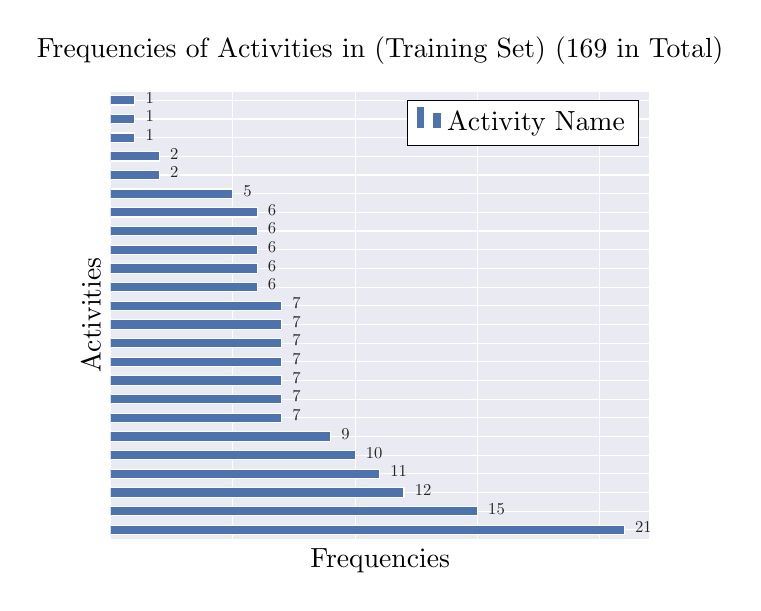
\begin{tikzpicture}

\definecolor{color0}{rgb}{0.917647058823529,0.917647058823529,0.949019607843137}
\definecolor{color1}{rgb}{0.298039215686275,0.447058823529412,0.690196078431373}

\begin{axis}[
axis background/.style={fill=color0},
axis line style={white},
tick align=outside,
title={Frequencies of Activities in (Training Set) (169 in Total)},
x grid style={white},
xlabel={Frequencies},
xmajorgrids,
xmajorticks=false,
xmin=0, xmax=22.05,
xtick style={color=white!15.0!black},
y grid style={white},
ylabel={Activities},
ymajorgrids,
ymajorticks=false,
ymin=-0.5, ymax=23.5,
ytick style={color=white!15.0!black},
ytick={0,1,2,3,4,5,6,7,8,9,10,11,12,13,14,15,16,17,18,19,20,21,22,23},
yticklabels={Brush teeth,Dressing,Enter the SmartLab ,Put waste in the bin ,Use the toilet,Leave the SmartLab,Take medication ,Breakfast,Dinner,Prepare breakfast,Prepare dinner ,Wake up,Go to the bed,Watch TV,Wash hands,Prepare lunch,Put washing into the washing machine,Lunch,Eat a snack,Wash dishes,Work at the table ,Relax on the sofa ,Visit in the SmartLab ,Play a videogame }
]
\draw[draw=white,fill=color1] (axis cs:0,-0.25) rectangle (axis cs:21,0.25);
\addlegendimage{ybar,ybar legend,draw=white,fill=color1};
\addlegendentry{Activity Name}

\draw[draw=white,fill=color1] (axis cs:0,0.75) rectangle (axis cs:15,1.25);
\draw[draw=white,fill=color1] (axis cs:0,1.75) rectangle (axis cs:12,2.25);
\draw[draw=white,fill=color1] (axis cs:0,2.75) rectangle (axis cs:11,3.25);
\draw[draw=white,fill=color1] (axis cs:0,3.75) rectangle (axis cs:10,4.25);
\draw[draw=white,fill=color1] (axis cs:0,4.75) rectangle (axis cs:9,5.25);
\draw[draw=white,fill=color1] (axis cs:0,5.75) rectangle (axis cs:7,6.25);
\draw[draw=white,fill=color1] (axis cs:0,6.75) rectangle (axis cs:7,7.25);
\draw[draw=white,fill=color1] (axis cs:0,7.75) rectangle (axis cs:7,8.25);
\draw[draw=white,fill=color1] (axis cs:0,8.75) rectangle (axis cs:7,9.25);
\draw[draw=white,fill=color1] (axis cs:0,9.75) rectangle (axis cs:7,10.25);
\draw[draw=white,fill=color1] (axis cs:0,10.75) rectangle (axis cs:7,11.25);
\draw[draw=white,fill=color1] (axis cs:0,11.75) rectangle (axis cs:7,12.25);
\draw[draw=white,fill=color1] (axis cs:0,12.75) rectangle (axis cs:6,13.25);
\draw[draw=white,fill=color1] (axis cs:0,13.75) rectangle (axis cs:6,14.25);
\draw[draw=white,fill=color1] (axis cs:0,14.75) rectangle (axis cs:6,15.25);
\draw[draw=white,fill=color1] (axis cs:0,15.75) rectangle (axis cs:6,16.25);
\draw[draw=white,fill=color1] (axis cs:0,16.75) rectangle (axis cs:6,17.25);
\draw[draw=white,fill=color1] (axis cs:0,17.75) rectangle (axis cs:5,18.25);
\draw[draw=white,fill=color1] (axis cs:0,18.75) rectangle (axis cs:2,19.25);
\draw[draw=white,fill=color1] (axis cs:0,19.75) rectangle (axis cs:2,20.25);
\draw[draw=white,fill=color1] (axis cs:0,20.75) rectangle (axis cs:1,21.25);
\draw[draw=white,fill=color1] (axis cs:0,21.75) rectangle (axis cs:1,22.25);
\draw[draw=white,fill=color1] (axis cs:0,22.75) rectangle (axis cs:1,23.25);
\draw[] (axis cs:21.2,-0.15) -- (axis cs:21.2,-0.15);
\node at (axis cs:21.2,-0.15)[
  scale=0.6,
  anchor=base west,
  text=white!15.0!black,
  rotate=0.0
]{21};
\draw[] (axis cs:15.2,0.85) -- (axis cs:15.2,0.85);
\node at (axis cs:15.2,0.85)[
  scale=0.6,
  anchor=base west,
  text=white!15.0!black,
  rotate=0.0
]{15};
\draw[] (axis cs:12.2,1.85) -- (axis cs:12.2,1.85);
\node at (axis cs:12.2,1.85)[
  scale=0.6,
  anchor=base west,
  text=white!15.0!black,
  rotate=0.0
]{12};
\draw[] (axis cs:11.2,2.85) -- (axis cs:11.2,2.85);
\node at (axis cs:11.2,2.85)[
  scale=0.6,
  anchor=base west,
  text=white!15.0!black,
  rotate=0.0
]{11};
\draw[] (axis cs:10.2,3.85) -- (axis cs:10.2,3.85);
\node at (axis cs:10.2,3.85)[
  scale=0.6,
  anchor=base west,
  text=white!15.0!black,
  rotate=0.0
]{10};
\draw[] (axis cs:9.2,4.85) -- (axis cs:9.2,4.85);
\node at (axis cs:9.2,4.85)[
  scale=0.6,
  anchor=base west,
  text=white!15.0!black,
  rotate=0.0
]{9};
\draw[] (axis cs:7.2,5.85) -- (axis cs:7.2,5.85);
\node at (axis cs:7.2,5.85)[
  scale=0.6,
  anchor=base west,
  text=white!15.0!black,
  rotate=0.0
]{7};
\draw[] (axis cs:7.2,6.85) -- (axis cs:7.2,6.85);
\node at (axis cs:7.2,6.85)[
  scale=0.6,
  anchor=base west,
  text=white!15.0!black,
  rotate=0.0
]{7};
\draw[] (axis cs:7.2,7.85) -- (axis cs:7.2,7.85);
\node at (axis cs:7.2,7.85)[
  scale=0.6,
  anchor=base west,
  text=white!15.0!black,
  rotate=0.0
]{7};
\draw[] (axis cs:7.2,8.85) -- (axis cs:7.2,8.85);
\node at (axis cs:7.2,8.85)[
  scale=0.6,
  anchor=base west,
  text=white!15.0!black,
  rotate=0.0
]{7};
\draw[] (axis cs:7.2,9.85) -- (axis cs:7.2,9.85);
\node at (axis cs:7.2,9.85)[
  scale=0.6,
  anchor=base west,
  text=white!15.0!black,
  rotate=0.0
]{7};
\draw[] (axis cs:7.2,10.85) -- (axis cs:7.2,10.85);
\node at (axis cs:7.2,10.85)[
  scale=0.6,
  anchor=base west,
  text=white!15.0!black,
  rotate=0.0
]{7};
\draw[] (axis cs:7.2,11.85) -- (axis cs:7.2,11.85);
\node at (axis cs:7.2,11.85)[
  scale=0.6,
  anchor=base west,
  text=white!15.0!black,
  rotate=0.0
]{7};
\draw[] (axis cs:6.2,12.85) -- (axis cs:6.2,12.85);
\node at (axis cs:6.2,12.85)[
  scale=0.6,
  anchor=base west,
  text=white!15.0!black,
  rotate=0.0
]{6};
\draw[] (axis cs:6.2,13.85) -- (axis cs:6.2,13.85);
\node at (axis cs:6.2,13.85)[
  scale=0.6,
  anchor=base west,
  text=white!15.0!black,
  rotate=0.0
]{6};
\draw[] (axis cs:6.2,14.85) -- (axis cs:6.2,14.85);
\node at (axis cs:6.2,14.85)[
  scale=0.6,
  anchor=base west,
  text=white!15.0!black,
  rotate=0.0
]{6};
\draw[] (axis cs:6.2,15.85) -- (axis cs:6.2,15.85);
\node at (axis cs:6.2,15.85)[
  scale=0.6,
  anchor=base west,
  text=white!15.0!black,
  rotate=0.0
]{6};
\draw[] (axis cs:6.2,16.85) -- (axis cs:6.2,16.85);
\node at (axis cs:6.2,16.85)[
  scale=0.6,
  anchor=base west,
  text=white!15.0!black,
  rotate=0.0
]{6};
\draw[] (axis cs:5.2,17.85) -- (axis cs:5.2,17.85);
\node at (axis cs:5.2,17.85)[
  scale=0.6,
  anchor=base west,
  text=white!15.0!black,
  rotate=0.0
]{5};
\draw[] (axis cs:2.2,18.85) -- (axis cs:2.2,18.85);
\node at (axis cs:2.2,18.85)[
  scale=0.6,
  anchor=base west,
  text=white!15.0!black,
  rotate=0.0
]{2};
\draw[] (axis cs:2.2,19.85) -- (axis cs:2.2,19.85);
\node at (axis cs:2.2,19.85)[
  scale=0.6,
  anchor=base west,
  text=white!15.0!black,
  rotate=0.0
]{2};
\draw[] (axis cs:1.2,20.85) -- (axis cs:1.2,20.85);
\node at (axis cs:1.2,20.85)[
  scale=0.6,
  anchor=base west,
  text=white!15.0!black,
  rotate=0.0
]{1};
\draw[] (axis cs:1.2,21.85) -- (axis cs:1.2,21.85);
\node at (axis cs:1.2,21.85)[
  scale=0.6,
  anchor=base west,
  text=white!15.0!black,
  rotate=0.0
]{1};
\draw[] (axis cs:1.2,22.85) -- (axis cs:1.2,22.85);
\node at (axis cs:1.2,22.85)[
  scale=0.6,
  anchor=base west,
  text=white!15.0!black,
  rotate=0.0
]{1};
\end{axis}

\end{tikzpicture}
